\documentclass[uplatex, dvipdfmx, a4paper, 10pt]{jsarticle}

\usepackage[top=15truemm,bottom=15truemm,left=18truemm,right=18truemm]{geometry}
\usepackage{amsmath, amssymb, mathtools, bm}
\usepackage[dvipdfmx]{graphicx}
\usepackage{float}
\usepackage{booktabs}
\usepackage{caption}
\usepackage[dvipdfmx, bookmarks=true, setpagesize=false, colorlinks=true, linkcolor=black, urlcolor=blue, citecolor=black]{hyperref}
\usepackage{pxjahyper}
\usepackage{listings}
\usepackage{xcolor}
\usepackage{tabularx}
\usepackage{enumitem}
\usepackage{multicol}

\definecolor{codegreen}{rgb}{0,0.6,0}
\definecolor{codegray}{rgb}{0.5,0.5,0.5}
\definecolor{codepurple}{rgb}{0.58,0,0.82}
\definecolor{backcolour}{rgb}{0.95,0.95,0.92}
\lstdefinestyle{mystyle}{
    backgroundcolor=\color{backcolour},
    commentstyle=\color{codegreen},
    keywordstyle=\color{magenta},
    numberstyle=\tiny\color{codegray},
    stringstyle=\color{codepurple},
    basicstyle=\ttfamily\scriptsize,
    breakatwhitespace=false, breaklines=true,
    captionpos=b, keepspaces=true,
    numbers=left, numbersep=4pt,
    showspaces=false, showstringspaces=false, showtabs=false,
    tabsize=2, frame=single,
    aboveskip=3pt, belowskip=1pt
}
\lstset{style=mystyle}

\newcommand{\ns}{\textrm{\scriptsize n.s.}}

\setlength{\parskip}{0.5pt plus 0.3pt}
\setlength{\abovecaptionskip}{2pt}
\setlength{\belowcaptionskip}{0pt}
\setlength{\floatsep}{2pt plus 1pt minus 1pt}
\setlength{\textfloatsep}{3pt plus 1pt minus 1pt}
\setlength{\intextsep}{2pt plus 1pt minus 1pt}
\setlist{nosep, leftmargin=1.5em, topsep=0pt, partopsep=0pt}
\captionsetup{font=small, skip=1pt}

\makeatletter
\renewcommand{\section}{\@startsection{section}{1}{\z@}%
    {0.5\Cvs \@plus.15\Cvs \@minus.05\Cvs}%
    {0.1\Cvs \@plus.05\Cvs}%
    {\normalfont\large\headfont\raggedright}}
\renewcommand{\subsection}{\@startsection{subsection}{2}{\z@}%
    {0.3\Cvs \@plus.1\Cvs \@minus.05\Cvs}%
    {0.05\Cvs \@plus.03\Cvs}{\normalfont\normalsize\headfont\raggedright}}
\makeatother

\title{\vspace{-10mm}データドリブン 第一回講義課題\\ \normalsize 履修者アンケートの定量的分析 By 鈴木真理\vspace{1mm}\\ \normalsize 履修者アンケートの定量分析By Gemini\vspace{1mm}}
\author{\small 慶應義塾大学 総合政策学部\quad 学籍番号: 72603857\quad 鈴木 真理}
\date{\small \today}

\newcommand{\point}[2]{\noindent\textbf{#1：} #2 \par}
\newcommand{\hypo}[1]{\item \textit{#1}} 

\begin{document}
\maketitle
\vspace{-7mm}

\begin{abstract}\small\setlength{\parskip}{0pt}
    本レポートは履修登録アンケート（n=912）に対し，筆者自らによるNumPyを用いた実装分析と，生成AI（Gemini）による分析を並行して実施し，その結果を比較検証したものである．
\end{abstract}

\section{分析結果の比較：筆者 vs Gemini}

\begin{multicols}{2}
    \subsection{筆者による分析}
    筆者は以下の3つの仮説を立て，NumPyを用いた独自実装により検証を行った．

    \begin{enumerate}[label=\textbf{\arabic*.}, nosep, leftmargin=2em]
        \item Python・SQL・R間に正の相関がある．
        \item 学部間でスキル差がある．
        \item 性別間でスキル差がある．
    \end{enumerate}
    \vspace{1em}
    \noindent \textbf{結果：} 仮説1と仮説3が支持された．

    \columnbreak

    \subsection{Geminiによる分析}
    Geminiは記述統計に基づき，データ全体の傾向を網羅的に集計した．

    \begin{enumerate}[label=\textbullet, nosep, leftmargin=2em]
        \item 全体の85\%がPython経験者である．
        \item 学部別の平均値に顕著な差はない．
    \end{enumerate}
    \vspace{1em}
    \noindent \textbf{特徴：} 表面的な記述統計に特化している．
\end{multicols}

\subsection{視覚的エビデンスによる仮説検証}

\begin{figure}[H]
    \centering
    \begin{minipage}{0.42\textwidth}
        \centering
        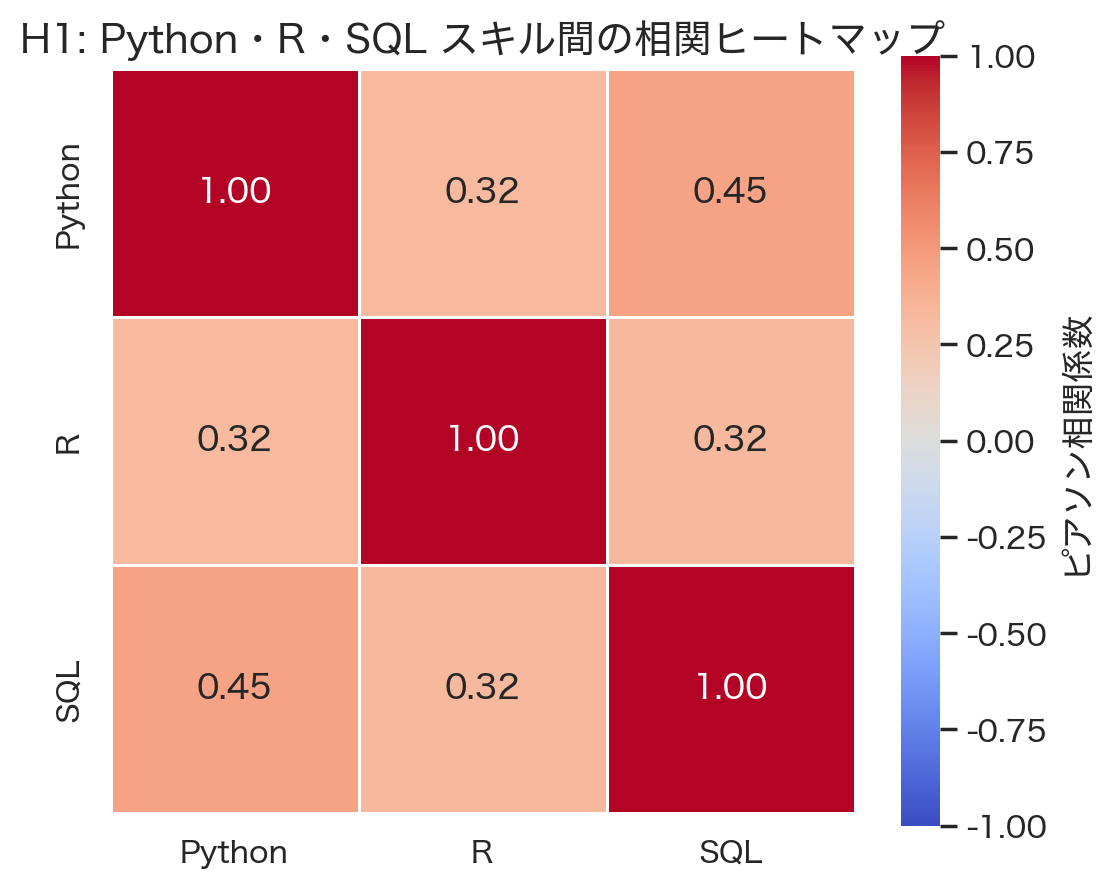
\includegraphics[width=\textwidth]{../Assets/h1_correlation_heatmap.png}
        %\caption{\footnotesize 相関行列(独自実装)}
        \label{fig:heatmap}
    \end{minipage}
    \hfill
    \begin{minipage}{0.45\textwidth}
        \centering
        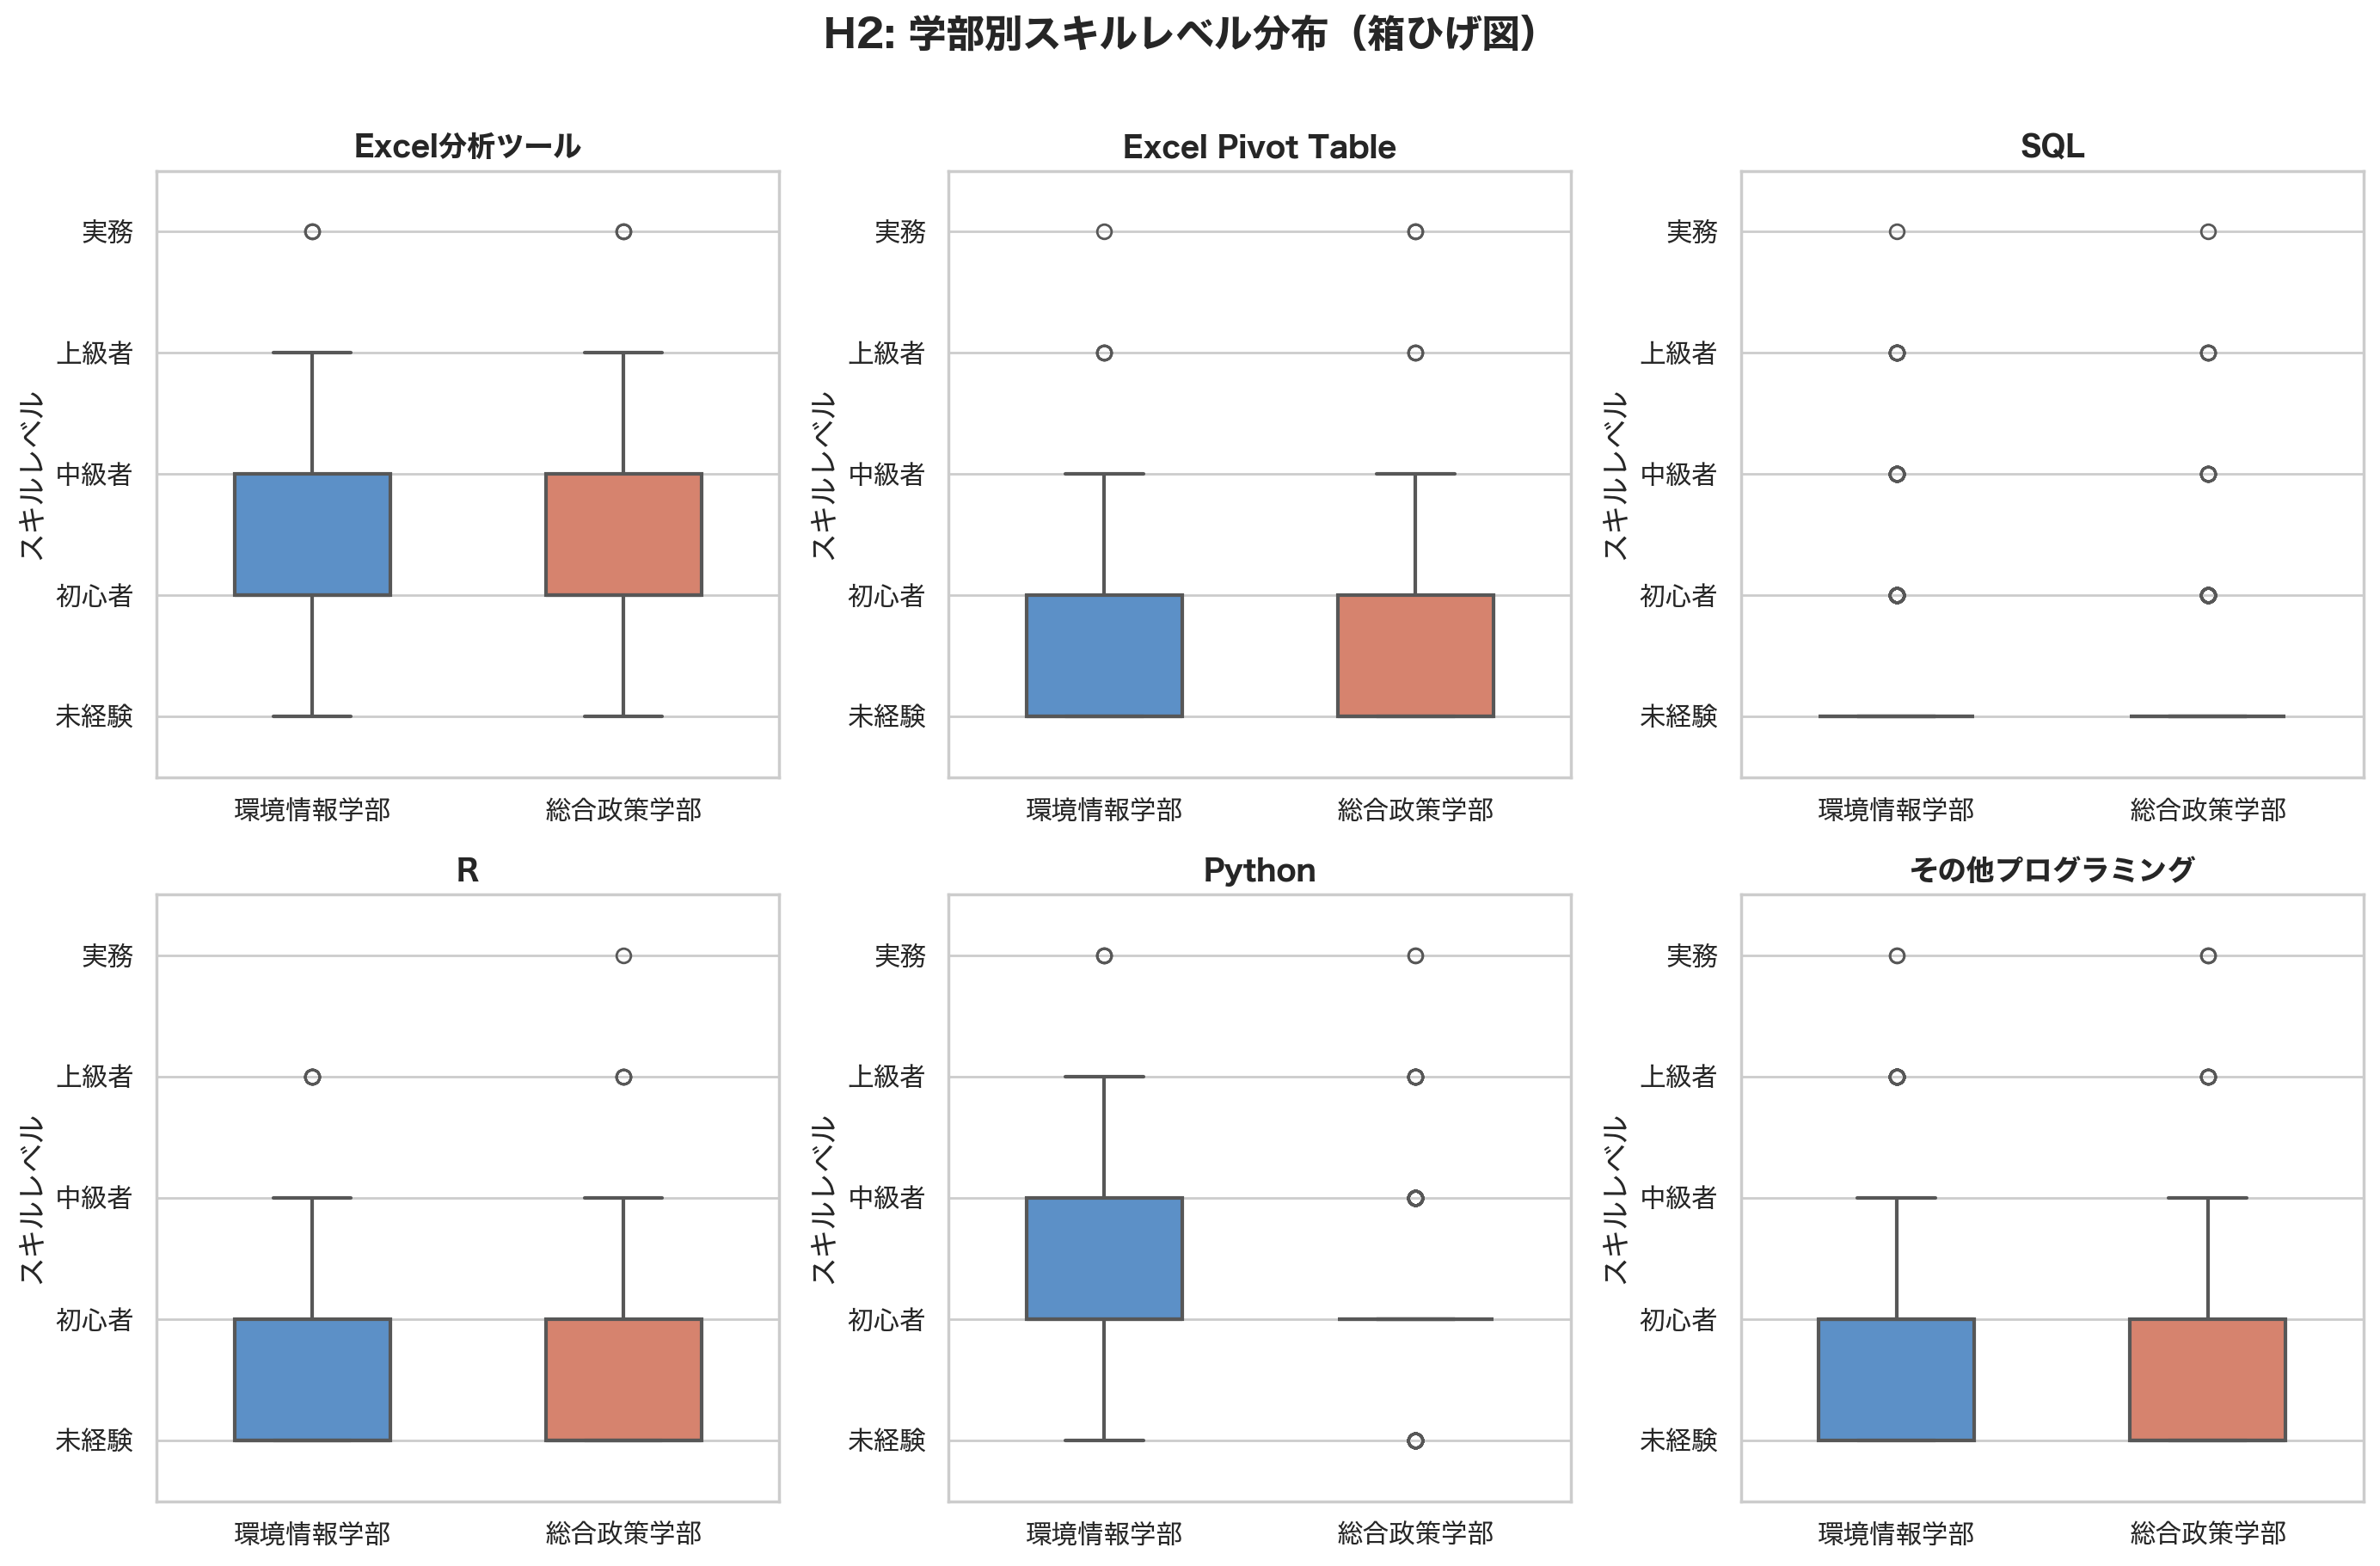
\includegraphics[width=\textwidth]{../Assets/h2_faculty_boxplot.png}
        %\caption{\footnotesize 学部別スキル分布}
        \label{fig:boxplot}
    \end{minipage}
    \hfill
    \begin{minipage}{0.42\textwidth}
        \centering
        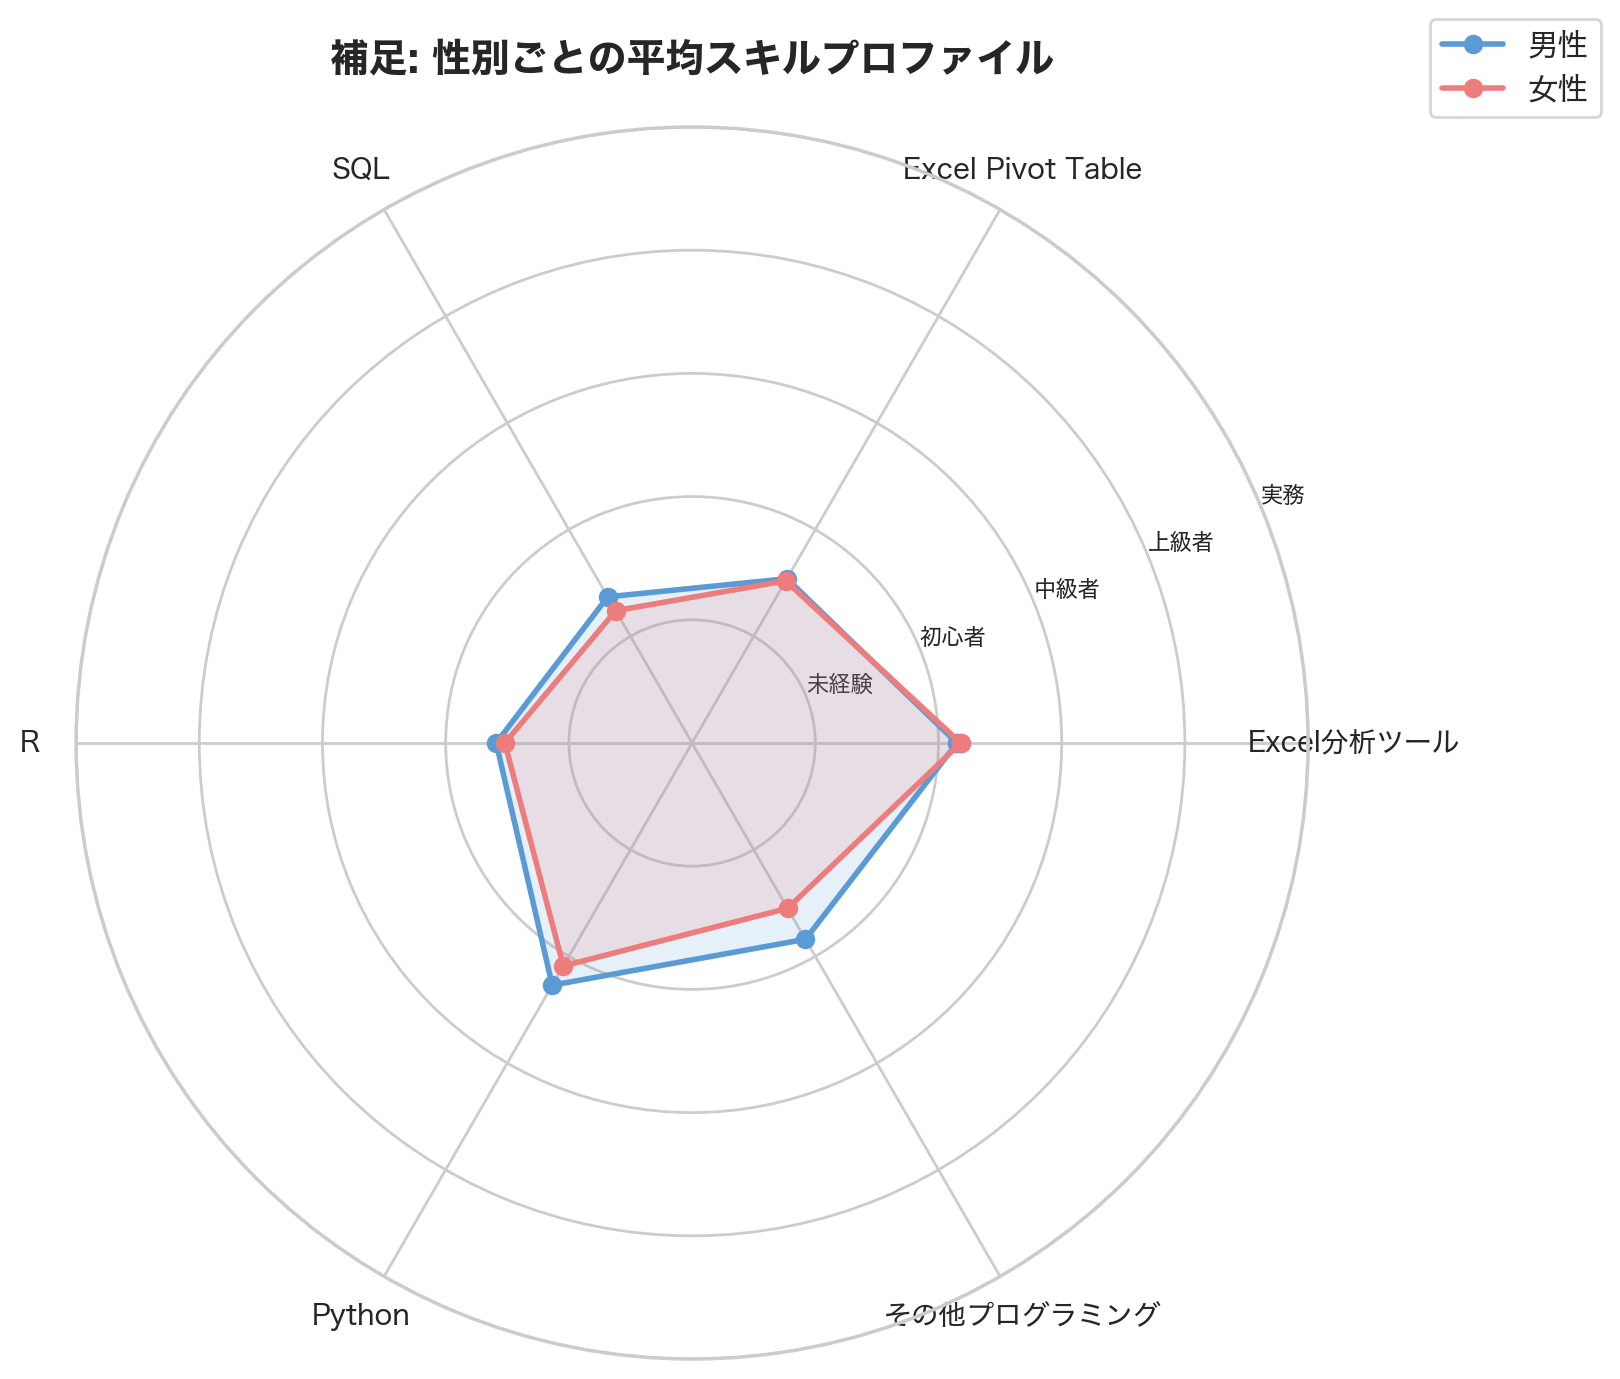
\includegraphics[width=\textwidth]{../Assets/h3_gender_radar.png}
        %\caption{\footnotesize 性別スキル偏差}
        \label{fig:radar}
    \end{minipage}
\end{figure}

\section{両者の比較と「つまらない分析」の正体}
\point{1. 分析結果の共通点}{
    \begin{itemize}[nosep]
        \hypo{Python経験者の割合が高い}
        \hypo{学部間のスキル差がない}
    \end{itemize}
}

\noindent\textbf{2. なぜ「つまらない」のか（考察）：}
\begin{itemize}
    \item \textbf{情報不足:}学生の学修環境や動機などの要素が考慮されていないため，スキルの背景にある要因を分析できない．
    \item \textbf{客観性がない:}本調査は主観的な評価に偏っているため，分析結果が個人の感覚に依存しやすく信憑性に欠ける．
    \item \textbf{前後比較が不能である:}初回授業という単一時点のデータのみであるため，スキルの成長や変化を追跡できない．
    \item \textbf{一定のバイアスがある:}履修選抜を突破できる学生が対象であるため，全体のスキル分布を正確に反映できない．
\end{itemize}

\section{意味合い（Insight）を出すための新たな問い}
現状を把握するだけの分析から脱却するため，以下の問いを設定する．
\begin{enumerate}
    \item \textbf{クラスター特性：} 個人によって
    \item \textbf{潜在的脱落者の予測：} 数学への苦手意識（1-2）とプログラミング経験の低さが結合している層に対し，どのタイミングで介入（スキャフォールディング）すべきか？
\end{enumerate}

\section{結論：この課題で本当に答えるべき問い}


\end{document}